% Options for packages loaded elsewhere
\PassOptionsToPackage{unicode}{hyperref}
\PassOptionsToPackage{hyphens}{url}
\PassOptionsToPackage{dvipsnames,svgnames,x11names}{xcolor}
%
\documentclass[
  letterpaper,
  DIV=11,
  numbers=noendperiod]{scrartcl}

\usepackage{amsmath,amssymb}
\usepackage{lmodern}
\usepackage{iftex}
\ifPDFTeX
  \usepackage[T1]{fontenc}
  \usepackage[utf8]{inputenc}
  \usepackage{textcomp} % provide euro and other symbols
\else % if luatex or xetex
  \usepackage{unicode-math}
  \defaultfontfeatures{Scale=MatchLowercase}
  \defaultfontfeatures[\rmfamily]{Ligatures=TeX,Scale=1}
\fi
% Use upquote if available, for straight quotes in verbatim environments
\IfFileExists{upquote.sty}{\usepackage{upquote}}{}
\IfFileExists{microtype.sty}{% use microtype if available
  \usepackage[]{microtype}
  \UseMicrotypeSet[protrusion]{basicmath} % disable protrusion for tt fonts
}{}
\makeatletter
\@ifundefined{KOMAClassName}{% if non-KOMA class
  \IfFileExists{parskip.sty}{%
    \usepackage{parskip}
  }{% else
    \setlength{\parindent}{0pt}
    \setlength{\parskip}{6pt plus 2pt minus 1pt}}
}{% if KOMA class
  \KOMAoptions{parskip=half}}
\makeatother
\usepackage{xcolor}
\setlength{\emergencystretch}{3em} % prevent overfull lines
\setcounter{secnumdepth}{-\maxdimen} % remove section numbering
% Make \paragraph and \subparagraph free-standing
\ifx\paragraph\undefined\else
  \let\oldparagraph\paragraph
  \renewcommand{\paragraph}[1]{\oldparagraph{#1}\mbox{}}
\fi
\ifx\subparagraph\undefined\else
  \let\oldsubparagraph\subparagraph
  \renewcommand{\subparagraph}[1]{\oldsubparagraph{#1}\mbox{}}
\fi

\usepackage{color}
\usepackage{fancyvrb}
\newcommand{\VerbBar}{|}
\newcommand{\VERB}{\Verb[commandchars=\\\{\}]}
\DefineVerbatimEnvironment{Highlighting}{Verbatim}{commandchars=\\\{\}}
% Add ',fontsize=\small' for more characters per line
\usepackage{framed}
\definecolor{shadecolor}{RGB}{241,243,245}
\newenvironment{Shaded}{\begin{snugshade}}{\end{snugshade}}
\newcommand{\AlertTok}[1]{\textcolor[rgb]{0.68,0.00,0.00}{#1}}
\newcommand{\AnnotationTok}[1]{\textcolor[rgb]{0.37,0.37,0.37}{#1}}
\newcommand{\AttributeTok}[1]{\textcolor[rgb]{0.40,0.45,0.13}{#1}}
\newcommand{\BaseNTok}[1]{\textcolor[rgb]{0.68,0.00,0.00}{#1}}
\newcommand{\BuiltInTok}[1]{\textcolor[rgb]{0.00,0.23,0.31}{#1}}
\newcommand{\CharTok}[1]{\textcolor[rgb]{0.13,0.47,0.30}{#1}}
\newcommand{\CommentTok}[1]{\textcolor[rgb]{0.37,0.37,0.37}{#1}}
\newcommand{\CommentVarTok}[1]{\textcolor[rgb]{0.37,0.37,0.37}{\textit{#1}}}
\newcommand{\ConstantTok}[1]{\textcolor[rgb]{0.56,0.35,0.01}{#1}}
\newcommand{\ControlFlowTok}[1]{\textcolor[rgb]{0.00,0.23,0.31}{#1}}
\newcommand{\DataTypeTok}[1]{\textcolor[rgb]{0.68,0.00,0.00}{#1}}
\newcommand{\DecValTok}[1]{\textcolor[rgb]{0.68,0.00,0.00}{#1}}
\newcommand{\DocumentationTok}[1]{\textcolor[rgb]{0.37,0.37,0.37}{\textit{#1}}}
\newcommand{\ErrorTok}[1]{\textcolor[rgb]{0.68,0.00,0.00}{#1}}
\newcommand{\ExtensionTok}[1]{\textcolor[rgb]{0.00,0.23,0.31}{#1}}
\newcommand{\FloatTok}[1]{\textcolor[rgb]{0.68,0.00,0.00}{#1}}
\newcommand{\FunctionTok}[1]{\textcolor[rgb]{0.28,0.35,0.67}{#1}}
\newcommand{\ImportTok}[1]{\textcolor[rgb]{0.00,0.46,0.62}{#1}}
\newcommand{\InformationTok}[1]{\textcolor[rgb]{0.37,0.37,0.37}{#1}}
\newcommand{\KeywordTok}[1]{\textcolor[rgb]{0.00,0.23,0.31}{#1}}
\newcommand{\NormalTok}[1]{\textcolor[rgb]{0.00,0.23,0.31}{#1}}
\newcommand{\OperatorTok}[1]{\textcolor[rgb]{0.37,0.37,0.37}{#1}}
\newcommand{\OtherTok}[1]{\textcolor[rgb]{0.00,0.23,0.31}{#1}}
\newcommand{\PreprocessorTok}[1]{\textcolor[rgb]{0.68,0.00,0.00}{#1}}
\newcommand{\RegionMarkerTok}[1]{\textcolor[rgb]{0.00,0.23,0.31}{#1}}
\newcommand{\SpecialCharTok}[1]{\textcolor[rgb]{0.37,0.37,0.37}{#1}}
\newcommand{\SpecialStringTok}[1]{\textcolor[rgb]{0.13,0.47,0.30}{#1}}
\newcommand{\StringTok}[1]{\textcolor[rgb]{0.13,0.47,0.30}{#1}}
\newcommand{\VariableTok}[1]{\textcolor[rgb]{0.07,0.07,0.07}{#1}}
\newcommand{\VerbatimStringTok}[1]{\textcolor[rgb]{0.13,0.47,0.30}{#1}}
\newcommand{\WarningTok}[1]{\textcolor[rgb]{0.37,0.37,0.37}{\textit{#1}}}

\providecommand{\tightlist}{%
  \setlength{\itemsep}{0pt}\setlength{\parskip}{0pt}}\usepackage{longtable,booktabs,array}
\usepackage{calc} % for calculating minipage widths
% Correct order of tables after \paragraph or \subparagraph
\usepackage{etoolbox}
\makeatletter
\patchcmd\longtable{\par}{\if@noskipsec\mbox{}\fi\par}{}{}
\makeatother
% Allow footnotes in longtable head/foot
\IfFileExists{footnotehyper.sty}{\usepackage{footnotehyper}}{\usepackage{footnote}}
\makesavenoteenv{longtable}
\usepackage{graphicx}
\makeatletter
\def\maxwidth{\ifdim\Gin@nat@width>\linewidth\linewidth\else\Gin@nat@width\fi}
\def\maxheight{\ifdim\Gin@nat@height>\textheight\textheight\else\Gin@nat@height\fi}
\makeatother
% Scale images if necessary, so that they will not overflow the page
% margins by default, and it is still possible to overwrite the defaults
% using explicit options in \includegraphics[width, height, ...]{}
\setkeys{Gin}{width=\maxwidth,height=\maxheight,keepaspectratio}
% Set default figure placement to htbp
\makeatletter
\def\fps@figure{htbp}
\makeatother

\KOMAoption{captions}{tableheading}
\makeatletter
\makeatother
\makeatletter
\makeatother
\makeatletter
\@ifpackageloaded{caption}{}{\usepackage{caption}}
\AtBeginDocument{%
\ifdefined\contentsname
  \renewcommand*\contentsname{Table of contents}
\else
  \newcommand\contentsname{Table of contents}
\fi
\ifdefined\listfigurename
  \renewcommand*\listfigurename{List of Figures}
\else
  \newcommand\listfigurename{List of Figures}
\fi
\ifdefined\listtablename
  \renewcommand*\listtablename{List of Tables}
\else
  \newcommand\listtablename{List of Tables}
\fi
\ifdefined\figurename
  \renewcommand*\figurename{Figure}
\else
  \newcommand\figurename{Figure}
\fi
\ifdefined\tablename
  \renewcommand*\tablename{Table}
\else
  \newcommand\tablename{Table}
\fi
}
\@ifpackageloaded{float}{}{\usepackage{float}}
\floatstyle{ruled}
\@ifundefined{c@chapter}{\newfloat{codelisting}{h}{lop}}{\newfloat{codelisting}{h}{lop}[chapter]}
\floatname{codelisting}{Listing}
\newcommand*\listoflistings{\listof{codelisting}{List of Listings}}
\makeatother
\makeatletter
\@ifpackageloaded{caption}{}{\usepackage{caption}}
\@ifpackageloaded{subcaption}{}{\usepackage{subcaption}}
\makeatother
\makeatletter
\@ifpackageloaded{tcolorbox}{}{\usepackage[many]{tcolorbox}}
\makeatother
\makeatletter
\@ifundefined{shadecolor}{\definecolor{shadecolor}{rgb}{.97, .97, .97}}
\makeatother
\makeatletter
\makeatother
\ifLuaTeX
  \usepackage{selnolig}  % disable illegal ligatures
\fi
\IfFileExists{bookmark.sty}{\usepackage{bookmark}}{\usepackage{hyperref}}
\IfFileExists{xurl.sty}{\usepackage{xurl}}{} % add URL line breaks if available
\urlstyle{same} % disable monospaced font for URLs
\hypersetup{
  pdftitle={Regresión Lineal},
  pdfauthor={Edmond Géraud},
  colorlinks=true,
  linkcolor={blue},
  filecolor={Maroon},
  citecolor={Blue},
  urlcolor={Blue},
  pdfcreator={LaTeX via pandoc}}

\title{Regresión Lineal}
\author{Edmond Géraud}
\date{}

\begin{document}
\maketitle
\ifdefined\Shaded\renewenvironment{Shaded}{\begin{tcolorbox}[enhanced, frame hidden, breakable, sharp corners, boxrule=0pt, interior hidden, borderline west={3pt}{0pt}{shadecolor}]}{\end{tcolorbox}}\fi

\hypertarget{estimaciuxf3n-del-peso-estuxe1ndar-del-huxedgado}{%
\section{Estimación del peso estándar del
hígado}\label{estimaciuxf3n-del-peso-estuxe1ndar-del-huxedgado}}

\begin{itemize}
\item
  gender
\item
  weight {[}kg{]}
\item
  height {[}cm{]}
\item
  liver\_weight {[}g{]}
\item
  liver\_volume {[}ml{]}
\end{itemize}

\begin{figure}

{\centering 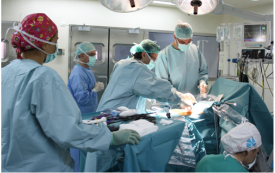
\includegraphics{Screenshot from 2023-04-16 20-01-51.png}

}

\caption{Intervención de cirugía hepática mayor por laparascopia}

\end{figure}

\hypertarget{necesitamos-cargar-las-libreruxedas}{%
\section{Necesitamos cargar las
librerías}\label{necesitamos-cargar-las-libreruxedas}}

\begin{Shaded}
\begin{Highlighting}[]
\ControlFlowTok{if}\NormalTok{ (}\SpecialCharTok{!}\NormalTok{(}\FunctionTok{require}\NormalTok{(car))) }\FunctionTok{install.packages}\NormalTok{(}\StringTok{"car"}\NormalTok{, }\AttributeTok{dep=}\ConstantTok{TRUE}\NormalTok{)}
\end{Highlighting}
\end{Shaded}

\begin{verbatim}
Loading required package: car
\end{verbatim}

\begin{verbatim}
Loading required package: carData
\end{verbatim}

\begin{Shaded}
\begin{Highlighting}[]
\ControlFlowTok{if}\NormalTok{ (}\SpecialCharTok{!}\NormalTok{(}\FunctionTok{require}\NormalTok{(DescTools))) }\FunctionTok{install.packages}\NormalTok{(}\StringTok{"DescTools"}\NormalTok{,}
                                            \AttributeTok{dependencies =}\NormalTok{ T)}
\end{Highlighting}
\end{Shaded}

\begin{verbatim}
Loading required package: DescTools
\end{verbatim}

\begin{verbatim}

Attaching package: 'DescTools'
\end{verbatim}

\begin{verbatim}
The following object is masked from 'package:car':

    Recode
\end{verbatim}

\begin{Shaded}
\begin{Highlighting}[]
\ControlFlowTok{if}\NormalTok{ (}\SpecialCharTok{!}\NormalTok{(}\FunctionTok{require}\NormalTok{(faraway))) }\FunctionTok{install.packages}\NormalTok{(}\StringTok{"DescTools"}\NormalTok{,}
                                            \AttributeTok{dependencies =}\NormalTok{ T)}
\end{Highlighting}
\end{Shaded}

\begin{verbatim}
Loading required package: faraway
\end{verbatim}

\begin{verbatim}

Attaching package: 'faraway'
\end{verbatim}

\begin{verbatim}
The following objects are masked from 'package:car':

    logit, vif
\end{verbatim}

\begin{Shaded}
\begin{Highlighting}[]
\NormalTok{ruta }\OtherTok{\textless{}{-}} \StringTok{"./data/chan\_data.csv"}
\NormalTok{datos }\OtherTok{\textless{}{-}} \FunctionTok{read.csv}\NormalTok{(ruta)}
\FunctionTok{class}\NormalTok{(datos)}
\end{Highlighting}
\end{Shaded}

\begin{verbatim}
[1] "data.frame"
\end{verbatim}

\begin{Shaded}
\begin{Highlighting}[]
\FunctionTok{str}\NormalTok{(datos)}
\end{Highlighting}
\end{Shaded}

\begin{verbatim}
'data.frame':   158 obs. of  5 variables:
 $ gender      : chr  "F" "F" "F" "F" ...
 $ weight      : num  50.3 47.4 44.3 44.1 52.1 51.3 51.8 42 52.1 44.1 ...
 $ height      : num  152 151 155 159 175 ...
 $ liver_weight: num  596 635 641 645 669 ...
 $ liver_volume: num  697 759 890 790 818 ...
\end{verbatim}

\hypertarget{cuxe1lculo-de-bmi-y-bsa-body-surface-area}{%
\subsubsection{Cálculo de BMI y BSA (body surface
area)}\label{cuxe1lculo-de-bmi-y-bsa-body-surface-area}}

\begin{Shaded}
\begin{Highlighting}[]
\NormalTok{logBSA }\OtherTok{\textless{}{-}}
\FunctionTok{log}\NormalTok{(}\FloatTok{0.007184}\NormalTok{) }\SpecialCharTok{+} \FloatTok{0.425} \SpecialCharTok{*} \FunctionTok{log}\NormalTok{(datos}\SpecialCharTok{$}\NormalTok{weight) }\SpecialCharTok{+} \FloatTok{0.725} \SpecialCharTok{*} \FunctionTok{log}\NormalTok{(datos}\SpecialCharTok{$}\NormalTok{height)}
\NormalTok{datos}\SpecialCharTok{$}\NormalTok{BSA }\OtherTok{\textless{}{-}} \FunctionTok{exp}\NormalTok{(logBSA)}
\NormalTok{datos}\SpecialCharTok{$}\NormalTok{BMI }\OtherTok{\textless{}{-}}\NormalTok{ datos}\SpecialCharTok{$}\NormalTok{weight}\SpecialCharTok{/}\NormalTok{(datos}\SpecialCharTok{$}\NormalTok{height}\SpecialCharTok{/}\DecValTok{100}\NormalTok{)}\SpecialCharTok{\^{}}\DecValTok{2}
\FunctionTok{str}\NormalTok{(datos)}
\end{Highlighting}
\end{Shaded}

\begin{verbatim}
'data.frame':   158 obs. of  7 variables:
 $ gender      : chr  "F" "F" "F" "F" ...
 $ weight      : num  50.3 47.4 44.3 44.1 52.1 51.3 51.8 42 52.1 44.1 ...
 $ height      : num  152 151 155 159 175 ...
 $ liver_weight: num  596 635 641 645 669 ...
 $ liver_volume: num  697 759 890 790 818 ...
 $ BSA         : num  1.45 1.41 1.39 1.42 1.63 ...
 $ BMI         : num  21.7 20.7 18.4 17.4 17 ...
\end{verbatim}

\hypertarget{quuxe9-es-necesario-saber-de-la-ols-y-mls}{%
\subsubsection{¿Qué es necesario saber de la OLS y
MLS?}\label{quuxe9-es-necesario-saber-de-la-ols-y-mls}}

\begin{enumerate}
\def\labelenumi{\arabic{enumi}.}
\item
  \[
  Y=X\beta+\epsilon
  \]

  \begin{itemize}
  \item
    La \(Y\) es la variable respuesta dependiente
  \item
    La \(X\) es/son las variables independientes
  \item
    La \(\epsilon\) es el error
  \end{itemize}
\item
  Supuestos

  \begin{itemize}
  \item
    \(\epsilon \sim N\)
  \item
    Linealidad: Al graficar no es una parábola por ejemplo
  \item
    Independencia, las variables deben ser independientes entre sí
  \item
    Homocedasticidad´
  \end{itemize}
\end{enumerate}

\hypertarget{estudiemos-la-normalidad-de-las-variables}{%
\subsubsection{Estudiemos la normalidad de las
variables}\label{estudiemos-la-normalidad-de-las-variables}}

Es una buena práctica realizar dichos análisis por motivos del modelo,
aunque no se cumplan la normalidad de las variables, es importante, que
una vez hecho el modelo, los residuos, es decir la diferencia entre la
variable respuesta y la predecida.

Lo podemos realizar de dos maneras, realizar un bucle for, o un apply

\begin{Shaded}
\begin{Highlighting}[]
\NormalTok{p.values }\OtherTok{\textless{}{-}} \FunctionTok{vector}\NormalTok{(}\StringTok{"numeric"}\NormalTok{,}\AttributeTok{length=}\FunctionTok{ncol}\NormalTok{(datos)}\SpecialCharTok{{-}}\DecValTok{1}\NormalTok{)}
\ControlFlowTok{for}\NormalTok{(i }\ControlFlowTok{in} \DecValTok{2}\SpecialCharTok{:}\FunctionTok{ncol}\NormalTok{(datos))\{}
  
  \FunctionTok{print}\NormalTok{(}\FunctionTok{paste}\NormalTok{(}\FunctionTok{round}\NormalTok{(}\FunctionTok{JarqueBeraTest}\NormalTok{(datos[,i])}\SpecialCharTok{$}\NormalTok{p.value,}\DecValTok{4}\NormalTok{),}\FunctionTok{colnames}\NormalTok{(datos)[i]))}
  
\NormalTok{\}}
\end{Highlighting}
\end{Shaded}

\begin{verbatim}
[1] "0.0824 weight"
[1] "0.1861 height"
[1] "0.0056 liver_weight"
[1] "0.0505 liver_volume"
[1] "0.0718 BSA"
[1] "4e-04 BMI"
\end{verbatim}

Es decir solamente el BMI y el peso del higado no siguen una normal.
Pero no hemos considerado los grupos por separado

\begin{Shaded}
\begin{Highlighting}[]
\FunctionTok{JarqueBeraTest}\NormalTok{(datos[datos}\SpecialCharTok{$}\NormalTok{gender}\SpecialCharTok{==}\StringTok{"F"}\NormalTok{,}\StringTok{"weight"}\NormalTok{])}
\end{Highlighting}
\end{Shaded}

\begin{verbatim}

    Robust Jarque Bera Test

data:  datos[datos$gender == "F", "weight"]
X-squared = 3.4764, df = 2, p-value = 0.1758
\end{verbatim}

\begin{Shaded}
\begin{Highlighting}[]
\FunctionTok{JarqueBeraTest}\NormalTok{(datos[datos}\SpecialCharTok{$}\NormalTok{gender}\SpecialCharTok{==}\StringTok{"M"}\NormalTok{,}\StringTok{"weight"}\NormalTok{])}
\end{Highlighting}
\end{Shaded}

\begin{verbatim}

    Robust Jarque Bera Test

data:  datos[datos$gender == "M", "weight"]
X-squared = 1.4866, df = 2, p-value = 0.4755
\end{verbatim}

\begin{Shaded}
\begin{Highlighting}[]
\FunctionTok{JarqueBeraTest}\NormalTok{(datos[datos}\SpecialCharTok{$}\NormalTok{gender}\SpecialCharTok{==}\StringTok{"M"}\NormalTok{,}\StringTok{"height"}\NormalTok{])}
\end{Highlighting}
\end{Shaded}

\begin{verbatim}

    Robust Jarque Bera Test

data:  datos[datos$gender == "M", "height"]
X-squared = 1.3449, df = 2, p-value = 0.5104
\end{verbatim}

\begin{Shaded}
\begin{Highlighting}[]
\FunctionTok{JarqueBeraTest}\NormalTok{(datos[datos}\SpecialCharTok{$}\NormalTok{gender}\SpecialCharTok{==}\StringTok{"M"}\NormalTok{,}\StringTok{"height"}\NormalTok{])}
\end{Highlighting}
\end{Shaded}

\begin{verbatim}

    Robust Jarque Bera Test

data:  datos[datos$gender == "M", "height"]
X-squared = 1.3449, df = 2, p-value = 0.5104
\end{verbatim}

Los cuatro test resultan no significativos y podemos considerar normales
estas dos variables en ambas poblaciones.

\hypertarget{regresiuxf3n-lineal-simple-ols}{%
\section{Regresión Lineal Simple
(OLS)}\label{regresiuxf3n-lineal-simple-ols}}

Procedemos a calcular la regresión del peso del hígado en función del
BSA

\begin{Shaded}
\begin{Highlighting}[]
\NormalTok{reg }\OtherTok{\textless{}{-}} \FunctionTok{lm}\NormalTok{(liver\_weight }\SpecialCharTok{\textasciitilde{}}\NormalTok{weight,}\AttributeTok{data=}\NormalTok{datos)}
\FunctionTok{summary}\NormalTok{(reg)}
\end{Highlighting}
\end{Shaded}

\begin{verbatim}

Call:
lm(formula = liver_weight ~ weight, data = datos)

Residuals:
    Min      1Q  Median      3Q     Max 
-254.39  -86.29   -9.92   66.44  396.58 

Coefficients:
            Estimate Std. Error t value Pr(>|t|)    
(Intercept)  141.725     71.419   1.984    0.049 *  
weight        14.043      1.254  11.195   <2e-16 ***
---
Signif. codes:  0 '***' 0.001 '**' 0.01 '*' 0.05 '.' 0.1 ' ' 1

Residual standard error: 131 on 156 degrees of freedom
Multiple R-squared:  0.4455,    Adjusted R-squared:  0.4419 
F-statistic: 125.3 on 1 and 156 DF,  p-value: < 2.2e-16
\end{verbatim}

Esto nos quiere decir, que por cada kilogramo de peso en las personas,
hay un incremento de 14 gramos en el peso del hígado.

\hypertarget{regresion-muxfaltiple}{%
\section{REGRESION MÚLTIPLE}\label{regresion-muxfaltiple}}

Ahora trabajaremos con el dataset \texttt{prostate} el cual se encuentra
en el paquete \texttt{faraway}. Este dataset donsiste en 97 filas y 9
columnas,los cuales se les realizo una prostatectomía

\begin{Shaded}
\begin{Highlighting}[]
\FunctionTok{summary}\NormalTok{(prostate)}
\end{Highlighting}
\end{Shaded}

\begin{verbatim}
     lcavol           lweight           age             lbph        
 Min.   :-1.3471   Min.   :2.375   Min.   :41.00   Min.   :-1.3863  
 1st Qu.: 0.5128   1st Qu.:3.376   1st Qu.:60.00   1st Qu.:-1.3863  
 Median : 1.4469   Median :3.623   Median :65.00   Median : 0.3001  
 Mean   : 1.3500   Mean   :3.653   Mean   :63.87   Mean   : 0.1004  
 3rd Qu.: 2.1270   3rd Qu.:3.878   3rd Qu.:68.00   3rd Qu.: 1.5581  
 Max.   : 3.8210   Max.   :6.108   Max.   :79.00   Max.   : 2.3263  
      svi              lcp             gleason          pgg45       
 Min.   :0.0000   Min.   :-1.3863   Min.   :6.000   Min.   :  0.00  
 1st Qu.:0.0000   1st Qu.:-1.3863   1st Qu.:6.000   1st Qu.:  0.00  
 Median :0.0000   Median :-0.7985   Median :7.000   Median : 15.00  
 Mean   :0.2165   Mean   :-0.1794   Mean   :6.753   Mean   : 24.38  
 3rd Qu.:0.0000   3rd Qu.: 1.1786   3rd Qu.:7.000   3rd Qu.: 40.00  
 Max.   :1.0000   Max.   : 2.9042   Max.   :9.000   Max.   :100.00  
      lpsa        
 Min.   :-0.4308  
 1st Qu.: 1.7317  
 Median : 2.5915  
 Mean   : 2.4784  
 3rd Qu.: 3.0564  
 Max.   : 5.5829  
\end{verbatim}

\begin{Shaded}
\begin{Highlighting}[]
\NormalTok{regr.pros }\OtherTok{\textless{}{-}} \FunctionTok{lm}\NormalTok{(lpsa}\SpecialCharTok{\textasciitilde{}}\NormalTok{lcavol}\SpecialCharTok{+}\NormalTok{lweight}\SpecialCharTok{+}\NormalTok{age}\SpecialCharTok{+}\NormalTok{lbph}\SpecialCharTok{+}\NormalTok{svi}\SpecialCharTok{+}\NormalTok{lcp}\SpecialCharTok{+}\NormalTok{gleason}\SpecialCharTok{+}\NormalTok{pgg45,prostate)}
\FunctionTok{summary}\NormalTok{(regr.pros)}
\end{Highlighting}
\end{Shaded}

\begin{verbatim}

Call:
lm(formula = lpsa ~ lcavol + lweight + age + lbph + svi + lcp + 
    gleason + pgg45, data = prostate)

Residuals:
    Min      1Q  Median      3Q     Max 
-1.7331 -0.3713 -0.0170  0.4141  1.6381 

Coefficients:
             Estimate Std. Error t value Pr(>|t|)    
(Intercept)  0.669337   1.296387   0.516  0.60693    
lcavol       0.587022   0.087920   6.677 2.11e-09 ***
lweight      0.454467   0.170012   2.673  0.00896 ** 
age         -0.019637   0.011173  -1.758  0.08229 .  
lbph         0.107054   0.058449   1.832  0.07040 .  
svi          0.766157   0.244309   3.136  0.00233 ** 
lcp         -0.105474   0.091013  -1.159  0.24964    
gleason      0.045142   0.157465   0.287  0.77503    
pgg45        0.004525   0.004421   1.024  0.30886    
---
Signif. codes:  0 '***' 0.001 '**' 0.01 '*' 0.05 '.' 0.1 ' ' 1

Residual standard error: 0.7084 on 88 degrees of freedom
Multiple R-squared:  0.6548,    Adjusted R-squared:  0.6234 
F-statistic: 20.86 on 8 and 88 DF,  p-value: < 2.2e-16
\end{verbatim}

\begin{Shaded}
\begin{Highlighting}[]
\FunctionTok{head}\NormalTok{(x0pros }\OtherTok{\textless{}{-}} \FunctionTok{data.frame}\NormalTok{(}\AttributeTok{lcavol=}\FloatTok{1.44692}\NormalTok{,}
                      \AttributeTok{lweight=}\FloatTok{3.62301}\NormalTok{,}
                      \AttributeTok{age=}\DecValTok{65}\NormalTok{,}
                      \AttributeTok{lbph=}\FloatTok{0.30010}\NormalTok{,}
                      \AttributeTok{svi=}\DecValTok{0}\NormalTok{,}
                      \AttributeTok{lcp=}\SpecialCharTok{{-}}\FloatTok{0.79851}\NormalTok{,}
                      \AttributeTok{gleason=}\DecValTok{7}\NormalTok{,}
                      \AttributeTok{pgg45=}\DecValTok{15}\NormalTok{))}
\end{Highlighting}
\end{Shaded}

\begin{verbatim}
   lcavol lweight age   lbph svi      lcp gleason pgg45
1 1.44692 3.62301  65 0.3001   0 -0.79851       7    15
\end{verbatim}

\begin{Shaded}
\begin{Highlighting}[]
 \FunctionTok{predict}\NormalTok{(regr.pros, x0pros, }\AttributeTok{interval=}\StringTok{"prediction"}\NormalTok{, }\AttributeTok{level=}\FloatTok{0.95}\NormalTok{) }
\end{Highlighting}
\end{Shaded}

\begin{verbatim}
       fit       lwr      upr
1 2.389053 0.9646584 3.813447
\end{verbatim}

El intervalo con el valor de 20 en \texttt{age} es más amplio que cuando
es 65 debido a que ese valor está fuera del rango de valores para esa
variables, y el modelo está extrapolando sobre valores que quedan fuera
de aquellos sobre los que se ha contruido el modelo de ajuste. Cuanto
más alejados sean los valores predictores de ese rango de valores
originales, más amplio será el intervalo, mayor el error y menos
ajustada la predicción.

\begin{Shaded}
\begin{Highlighting}[]
\FunctionTok{summary}\NormalTok{(regr.pros)}\SpecialCharTok{$}\NormalTok{coef[,}\DecValTok{4}\NormalTok{]}\SpecialCharTok{\textless{}}\FloatTok{0.05}
\end{Highlighting}
\end{Shaded}

\begin{verbatim}
(Intercept)      lcavol     lweight         age        lbph         svi 
      FALSE        TRUE        TRUE       FALSE       FALSE        TRUE 
        lcp     gleason       pgg45 
      FALSE       FALSE       FALSE 
\end{verbatim}

\begin{Shaded}
\begin{Highlighting}[]
 \FunctionTok{confint}\NormalTok{(regr.pros)}
\end{Highlighting}
\end{Shaded}

\begin{verbatim}
                   2.5 %      97.5 %
(Intercept) -1.906960983 3.245634379
lcavol       0.412298699 0.761744954
lweight      0.116603435 0.792331414
age         -0.041840618 0.002566267
lbph        -0.009101499 0.223209561
svi          0.280644232 1.251670420
lcp         -0.286344443 0.075395916
gleason     -0.267786053 0.358069248
pgg45       -0.004260932 0.013311395
\end{verbatim}

\begin{Shaded}
\begin{Highlighting}[]
\NormalTok{regr.pros2 }\OtherTok{\textless{}{-}} \FunctionTok{lm}\NormalTok{(lpsa}\SpecialCharTok{\textasciitilde{}}\NormalTok{lcavol}\SpecialCharTok{+}\NormalTok{lweight}\SpecialCharTok{+}\NormalTok{svi,prostate)}
\FunctionTok{summary}\NormalTok{(regr.pros2)}
\end{Highlighting}
\end{Shaded}

\begin{verbatim}

Call:
lm(formula = lpsa ~ lcavol + lweight + svi, data = prostate)

Residuals:
     Min       1Q   Median       3Q      Max 
-1.72964 -0.45764  0.02812  0.46403  1.57013 

Coefficients:
            Estimate Std. Error t value Pr(>|t|)    
(Intercept) -0.26809    0.54350  -0.493  0.62298    
lcavol       0.55164    0.07467   7.388  6.3e-11 ***
lweight      0.50854    0.15017   3.386  0.00104 ** 
svi          0.66616    0.20978   3.176  0.00203 ** 
---
Signif. codes:  0 '***' 0.001 '**' 0.01 '*' 0.05 '.' 0.1 ' ' 1

Residual standard error: 0.7168 on 93 degrees of freedom
Multiple R-squared:  0.6264,    Adjusted R-squared:  0.6144 
F-statistic: 51.99 on 3 and 93 DF,  p-value: < 2.2e-16
\end{verbatim}

\hypertarget{suposiciones}{%
\subsubsection{Suposiciones}\label{suposiciones}}

\hypertarget{varianza-constate}{%
\paragraph{Varianza constate}\label{varianza-constate}}

\begin{Shaded}
\begin{Highlighting}[]
\NormalTok{model }\OtherTok{\textless{}{-}} \FunctionTok{lm}\NormalTok{(lpsa}\SpecialCharTok{\textasciitilde{}}\NormalTok{lcavol}\SpecialCharTok{+}\NormalTok{lweight}\SpecialCharTok{+}\NormalTok{age}\SpecialCharTok{+}\NormalTok{lbph}\SpecialCharTok{+}\NormalTok{svi}\SpecialCharTok{+}\NormalTok{lcp}\SpecialCharTok{+}\NormalTok{gleason}\SpecialCharTok{+}\NormalTok{pgg45,prostate)}
\FunctionTok{plot}\NormalTok{(}\FunctionTok{fitted}\NormalTok{(model),}\FunctionTok{abs}\NormalTok{(}\FunctionTok{residuals}\NormalTok{(model)),}\AttributeTok{xlab=}\StringTok{"Predict values"}\NormalTok{,}\AttributeTok{ylab=}\StringTok{"|Residuals|"}\NormalTok{)}
\end{Highlighting}
\end{Shaded}

\begin{figure}[H]

{\centering 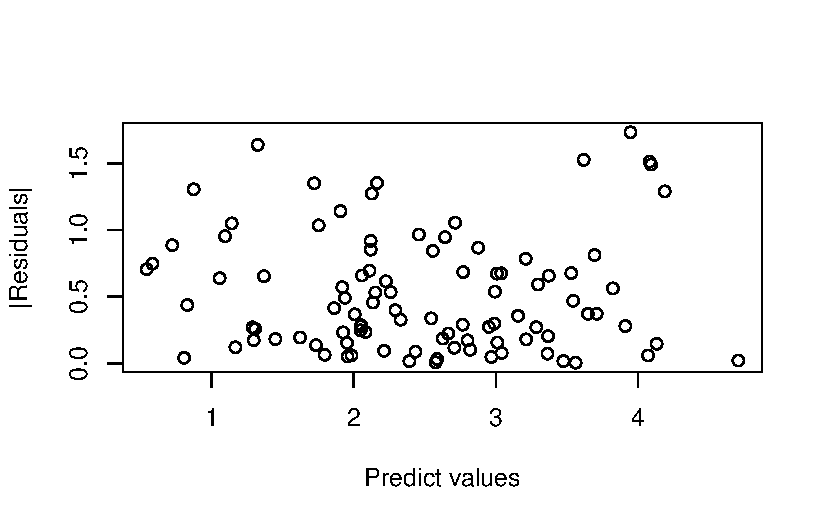
\includegraphics{Regresion-Lineal_files/figure-pdf/unnamed-chunk-15-1.pdf}

}

\end{figure}

\begin{Shaded}
\begin{Highlighting}[]
\FunctionTok{sumary}\NormalTok{(}\FunctionTok{lm}\NormalTok{(}\FunctionTok{sqrt}\NormalTok{(}\FunctionTok{abs}\NormalTok{(}\FunctionTok{residuals}\NormalTok{(model)))}\SpecialCharTok{\textasciitilde{}}\FunctionTok{fitted}\NormalTok{(model)))}
\end{Highlighting}
\end{Shaded}

\begin{verbatim}
               Estimate Std. Error t value  Pr(>|t|)
(Intercept)    0.703381   0.090607  7.7630 9.475e-12
fitted(model) -0.021990   0.034232 -0.6424    0.5222

n = 97, p = 2, Residual SE = 0.31328, R-Squared = 0
\end{verbatim}

No existen indicios de heterocedasticidad

\hypertarget{normalidad}{%
\paragraph{Normalidad}\label{normalidad}}

\begin{Shaded}
\begin{Highlighting}[]
\FunctionTok{qqnorm}\NormalTok{(}\FunctionTok{residuals}\NormalTok{(model),}\AttributeTok{ylab=}\StringTok{"Residus"}\NormalTok{)}
\FunctionTok{qqline}\NormalTok{(}\FunctionTok{residuals}\NormalTok{(model))}
\end{Highlighting}
\end{Shaded}

\begin{figure}[H]

{\centering 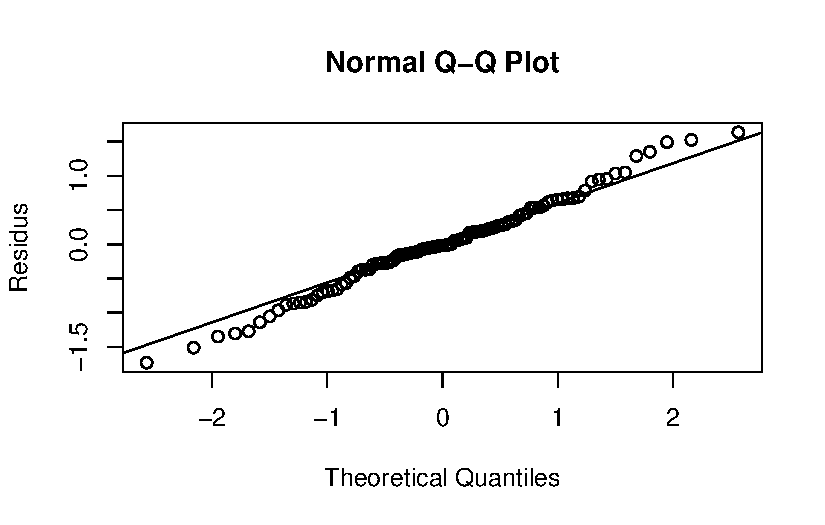
\includegraphics{Regresion-Lineal_files/figure-pdf/unnamed-chunk-17-1.pdf}

}

\end{figure}

\begin{Shaded}
\begin{Highlighting}[]
\FunctionTok{shapiro.test}\NormalTok{(}\FunctionTok{residuals}\NormalTok{(model))}
\end{Highlighting}
\end{Shaded}

\begin{verbatim}

    Shapiro-Wilk normality test

data:  residuals(model)
W = 0.99113, p-value = 0.7721
\end{verbatim}

Hay una cierta desviación respecto a la normal, con las colas algo
alargadas.

\hypertarget{leverage}{%
\paragraph{Leverage}\label{leverage}}

O influencia de los puntos

\begin{Shaded}
\begin{Highlighting}[]
\NormalTok{hatv }\OtherTok{\textless{}{-}} \FunctionTok{hatvalues}\NormalTok{(model)}
\FunctionTok{head}\NormalTok{(}\FunctionTok{sort}\NormalTok{(hatv,}\AttributeTok{decreasing=}\NormalTok{T))}
\end{Highlighting}
\end{Shaded}

\begin{verbatim}
       32        41        37        92        74        63 
0.3304757 0.2410079 0.2184392 0.2092421 0.1912109 0.1846807 
\end{verbatim}

\begin{Shaded}
\begin{Highlighting}[]
\NormalTok{p }\OtherTok{\textless{}{-}} \FunctionTok{length}\NormalTok{(model}\SpecialCharTok{$}\NormalTok{coefficients) }\CommentTok{\# k+1}
\NormalTok{n }\OtherTok{\textless{}{-}} \FunctionTok{length}\NormalTok{(model}\SpecialCharTok{$}\NormalTok{fitted.values)}
\FunctionTok{which}\NormalTok{(hatv }\SpecialCharTok{\textgreater{}} \DecValTok{2}\SpecialCharTok{*}\NormalTok{p}\SpecialCharTok{/}\NormalTok{n)}
\end{Highlighting}
\end{Shaded}

\begin{verbatim}
32 37 41 74 92 
32 37 41 74 92 
\end{verbatim}

\begin{Shaded}
\begin{Highlighting}[]
\FunctionTok{plot}\NormalTok{(hatv, }\AttributeTok{type=}\StringTok{"h"}\NormalTok{)}
 \FunctionTok{abline}\NormalTok{(}\AttributeTok{h=}\DecValTok{2}\SpecialCharTok{*}\NormalTok{p}\SpecialCharTok{/}\NormalTok{n, }\AttributeTok{col=}\StringTok{"red"}\NormalTok{)}
\end{Highlighting}
\end{Shaded}

\begin{figure}[H]

{\centering 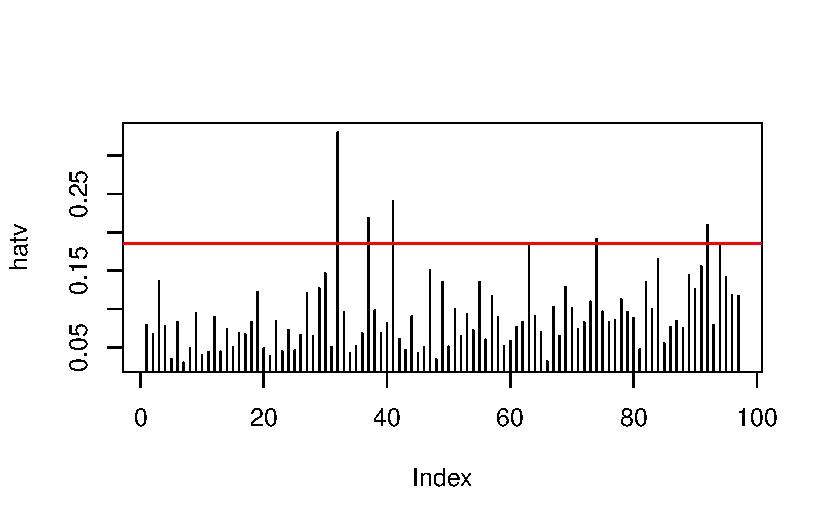
\includegraphics{Regresion-Lineal_files/figure-pdf/unnamed-chunk-21-1.pdf}

}

\end{figure}

\hypertarget{valores-atuxedpicos-u-outliers}{%
\paragraph{Valores atípicos u
outliers}\label{valores-atuxedpicos-u-outliers}}

\begin{Shaded}
\begin{Highlighting}[]
\NormalTok{stud }\OtherTok{\textless{}{-}} \FunctionTok{rstudent}\NormalTok{(model)}
\FunctionTok{which}\NormalTok{(}\FunctionTok{abs}\NormalTok{(stud) }\SpecialCharTok{\textgreater{}} \FunctionTok{abs}\NormalTok{(}\FunctionTok{qt}\NormalTok{(}\FloatTok{0.05}\SpecialCharTok{/}\NormalTok{(}\DecValTok{2}\SpecialCharTok{*}\NormalTok{n),}\AttributeTok{df=}\NormalTok{n}\SpecialCharTok{{-}}\NormalTok{p}\DecValTok{{-}1}\NormalTok{)))}
\end{Highlighting}
\end{Shaded}

\begin{verbatim}
named integer(0)
\end{verbatim}

\hypertarget{tarea}{%
\section{TAREA}\label{tarea}}

Leer y realizar resumen de pas pags 225-282, incluido el lab. En un
documento de Quarto.



\end{document}
